% ============================================================
%  CHAPTER 4: DESIGN AND IMPLEMENTATION
% ============================================================
\chapter{Design and Implementation}

This chapter describes the design and implementation of each component of the
Supply Chain Digital Twin. Section~4.1 lists the libraries and frameworks used.
Section~4.2 describes the simulation engine and the Nagpur road network.
Section~4.3 presents the full three-tier AI architecture. Section~4.4 covers the
PPO training procedure, including hyperparameters and the overfitting mitigation
strategy. Section~4.5 describes the Anti-Thrashing GPS Lock, which resolved a
critical fleet paralysis bug discovered during development.

% ================================================================
\section{System Components}

The system is divided into five major components that work together to form the
complete Digital Twin pipeline.

\begin{itemize}
    \item \textbf{Simulation Engine:} The core discrete-event engine that advances
    simulated time, generates orders, manages truck state, and injects environmental
    events such as weather changes and road accidents.
    \item \textbf{City Graph (NetworkX):} The weighted directed graph representing
    the Nagpur road network, on which all routing computations are performed.
    \item \textbf{Central PPO Brain:} The offline-trained macro-level routing agent.
    \item \textbf{Edge Q-Learning Agents:} Per-truck online agents for emergency
    micro-rerouting.
    \item \textbf{ETA Forecaster:} The online Ridge Regression model for
    spatial-temporal travel time prediction.
\end{itemize}

% ----------------------------------------------------------------
\subsection{Libraries and Frameworks}

Table~\ref{tab:libraries} lists the key libraries used in the implementation.

\begin{table}[h!]
\centering
\caption{Libraries and Frameworks Used}
\label{tab:libraries}
\begin{tabular}{|l|l|p{7cm}|}
\hline
\textbf{Library}          & \textbf{Version} & \textbf{Purpose} \\
\hline
Python                    & 3.10             & Primary implementation language \\
\hline
Stable-Baselines3         & 2.x              & PPO implementation, training loop, and EvalCallback \\
\hline
Gymnasium                 & 0.29             & Reinforcement learning environment interface (Env API) \\
\hline
NetworkX                  & 3.x              & Nagpur city graph construction, A* route planning \\
\hline
scikit-learn              & 1.4              & Ridge Regression ETA Forecaster with partial\_fit support \\
\hline
NumPy                     & 1.26             & State vector construction and numerical operations \\
\hline
Pandas                    & 2.x              & Telemetry CSV loading, event parsing, and analysis \\
\hline
PyYAML                    & 6.x              & Configuration management (simulation\_config.yaml) \\
\hline
Matplotlib                & 3.8              & Benchmark chart and thesis figure generation \\
\hline
\end{tabular}
\end{table}

% ================================================================
\section{Simulation Engine Architecture}

% ----------------------------------------------------------------
\subsection{Discrete-Event Simulation Loop}

The simulation engine advances time in discrete steps of 15 simulated minutes.
At each tick, the engine performs the following operations in sequence: it processes
all pending order placements from retailer nodes; it assigns available trucks to
orders using a fleet allocation algorithm; it advances the physical position of all
in-transit trucks along their current routes; it checks for and injects
environmental events (weather updates, road accidents, traffic density changes);
and it logs the state of every truck to the telemetry CSV file.

Figure~\ref{fig:order_lifecycle} shows the full lifecycle of an order from
placement through delivery. The sequence of events is strictly deterministic for
a given random seed, which allows the baseline and RL runs to be compared under
identical conditions.

\begin{figure}[h!]
    \centering
    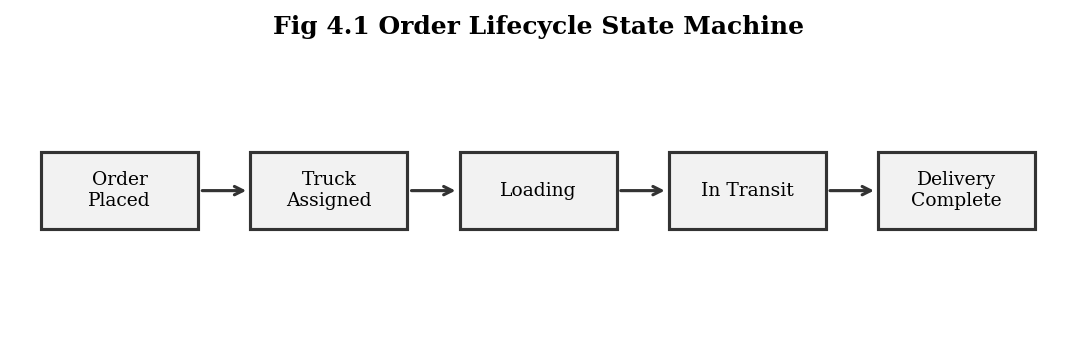
\includegraphics[width=0.98\textwidth]{images/fig4_1_order_lifecycle.png}
    \caption{Order Lifecycle State Machine from Placement to Delivery Completion}
    \label{fig:order_lifecycle}
\end{figure}

% ----------------------------------------------------------------
\subsection{Nagpur Road Network and A* Base Planner}

The road network is represented as a weighted directed graph using the NetworkX
library. The A* algorithm serves as the base route planner within the simulation.
Its edge cost function is parameterized by the routing strategy currently assigned
to the truck by the Central PPO Brain. Under Fuel-Priority mode, edge costs are
proportional to estimated fuel consumption per segment. Under RSL-Priority mode,
costs are proportional to estimated travel time. Under Speed-Priority mode, costs
combine time and a zone-based penalty that penalizes segments in congested zones
during peak hours.

% ----------------------------------------------------------------
\subsection{Dynamic Environmental Events}

Weather conditions are updated at the start of each simulated day, drawing from a
seasonal probability distribution calibrated to Nagpur's climate. The monsoon
months (June through September) have a high probability of rainfall, which
increases edge weights in all zones. Extreme summer heat (April through June)
increases cargo decay rates. Road accidents are injected as random events on
individual edges, temporarily increasing the cost of traversal. The Edge Q-Agent
is triggered whenever an accident is detected on a truck's current planned route.

% ================================================================
\section{Three-Tier AI Architecture}

% ----------------------------------------------------------------
\subsection{Architecture Overview}

Figure~\ref{fig:architecture} shows the full three-tier architecture and the data
flow between components.

\begin{figure}[h!]
    \centering
    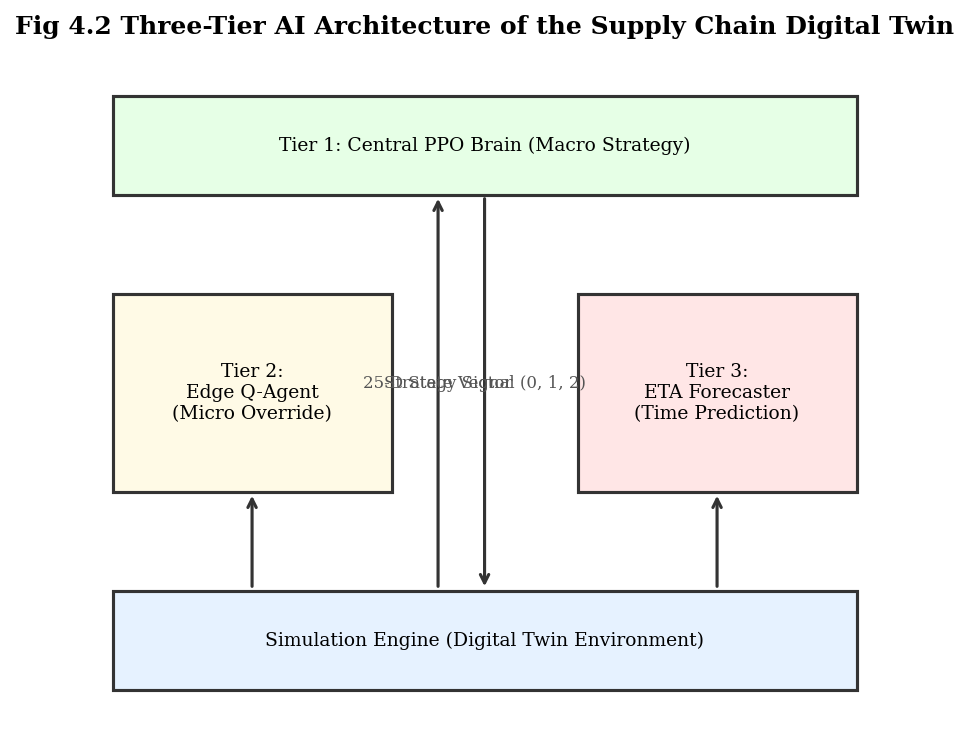
\includegraphics[width=0.92\textwidth]{images/fig4_2_architecture.png}
    \caption{Three-Tier AI Architecture of the Supply Chain Digital Twin}
    \label{fig:architecture}
\end{figure}

% ----------------------------------------------------------------
\subsection{Tier 1: Central PPO Brain (Macro Routing)}

The Central PPO Brain is the primary intelligence of the system. It is implemented
using the Stable-Baselines3 library \cite{stable_baselines3}, which provides a
production-quality implementation of the PPO algorithm. The brain is trained
offline for 50,000 steps before the benchmark phase begins, and during the
benchmark it operates in inference-only mode (the model weights are frozen and
only forward passes are performed).

The observation space is defined as \texttt{Box(25,)} with all values in $[0, 1]$.
The action space is \texttt{Discrete(3)}, representing the three routing strategies.
The neural network policy is a Multi-Layer Perceptron (MLP) with two hidden layers
of 64 neurons each and ReLU activation functions.

% ----------------------------------------------------------------
\subsection{Tier 2: Edge Q-Learning Emergency Agent (Micro Rerouting)}

Each truck in the fleet carries a separate Edge Q-Agent. The agent is implemented
as a tabular Q-learner with a small discrete state space representing the local
hazard context: the severity of the detected emergency (low, medium, high) and the
number of viable alternate routes available at the current position. This results
in a $3 \times 3 = 9$-state Q-table with 2 possible actions (attempt alternate
route, or wait for clearance).

The agent uses an epsilon-greedy exploration policy with $\epsilon$ decaying from
0.5 to 0.05 over 1,000 emergency events. After each emergency is resolved, the
Q-table is updated using the standard Bellman equation with learning rate $\alpha
= 0.1$ and discount factor $\gamma = 0.9$. The Edge Agent overrides the Central
Brain's routing strategy during the emergency and relinquishes control once the
truck has successfully cleared the blocked segment.

% ----------------------------------------------------------------
\subsection{Tier 3: ETA Forecaster (Online Ridge Regression)}

The ETA Forecaster is implemented using scikit-learn's \texttt{SGDRegressor} with
an L2 (Ridge) penalty. After each road segment is traversed by any truck, the
actual traversal time is recorded and used as a training sample to update the model
via \texttt{partial\_fit()}. This online learning loop means the model continuously
improves its predictions as the simulation accumulates real traversal data across
all zones, times of day, and weather conditions.

The 8-dimensional feature vector is constructed for each segment traversal as
described in Chapter~3. The predicted travel time returned by the model is injected
into the A* edge cost function, replacing the static average-based estimate used
in the baseline configuration.

\begin{figure}[htbp]
    \centering
    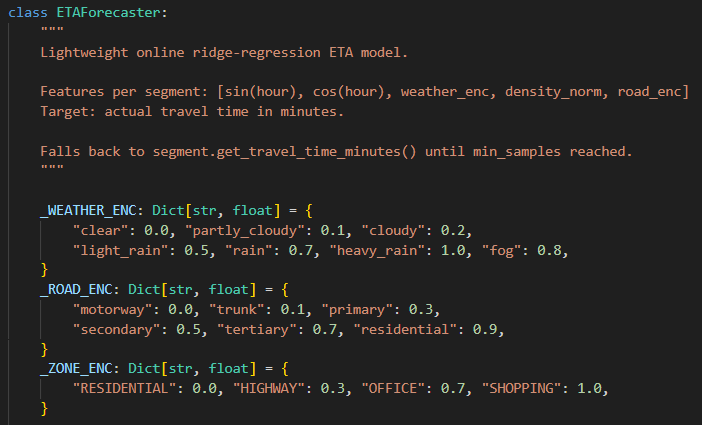
\includegraphics[width=0.95\textwidth, height=0.4\textheight, keepaspectratio]{images/screenshot_eta_forecaster_1.png}
    \vspace{0.2cm}
    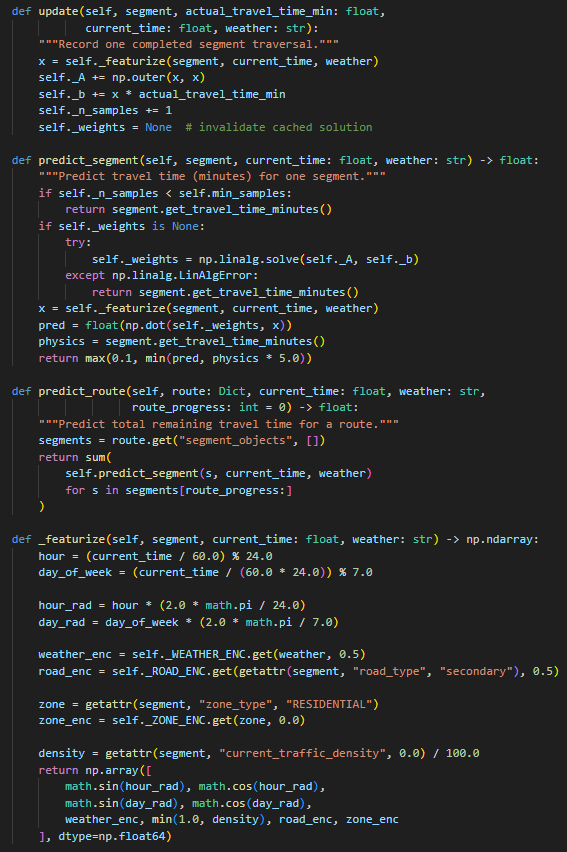
\includegraphics[width=0.95\textwidth, height=0.4\textheight, keepaspectratio]{images/screenshot_eta_forecaster_2.png}
    \caption{Implementation of the ETA Forecaster with 8-Dimensional Feature Vector (Part 1 \& 2)}
    \label{fig:eta_code}
\end{figure}

% ================================================================
\section{PPO Training Procedure}

% ----------------------------------------------------------------
\subsection{Routing Environment (RoutingEnv)}

The training environment is implemented as a custom Gymnasium \texttt{Env} subclass
named \texttt{RoutingEnv}. The \texttt{reset()} method initializes the simulation
at the start of a new training episode. The \texttt{step(a)} method advances the
simulation by one dispatch cycle, applies the selected strategy $a$, computes the
reward, and returns the next observation. The environment is registered with
Gymnasium and wrapped with a \texttt{Monitor} wrapper that logs episode rewards
and lengths to a file for analysis.

\begin{figure}[htbp]
    \centering
    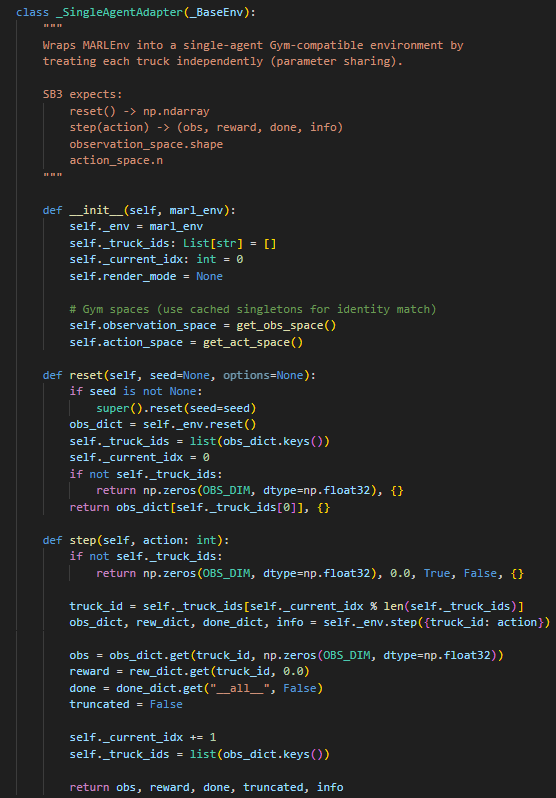
\includegraphics[width=0.95\textwidth, height=0.5\textheight, keepaspectratio]{images/screenshot_ppo_env.png}
    \caption{Single-Agent Gymnasium Environment Adapter for the Central PPO Brain}
    \label{fig:ppo_env_code}
\end{figure}

% ----------------------------------------------------------------
\subsection{Hyperparameters and Training Configuration}

Table~\ref{tab:ppo_hyperparams} lists all hyperparameters used for PPO training.

\begin{table}[h!]
\centering
\caption{PPO Training Hyperparameters}
\label{tab:ppo_hyperparams}
\begin{tabular}{|l|l|p{6cm}|}
\hline
\textbf{Hyperparameter} & \textbf{Value} & \textbf{Rationale} \\
\hline
Total timesteps         & 50,000         & Sufficient for convergence on a 3-action discrete problem \\
\hline
Learning rate           & 0.0003         & Standard PPO default; stable for MLP policies \\
\hline
n\_steps                & 2,048          & Rollout buffer size; balances variance and bias \\
\hline
batch\_size             & 64             & Mini-batch size for gradient updates \\
\hline
n\_epochs               & 10             & Number of optimization epochs per rollout \\
\hline
ent\_coef               & 0.01           & Entropy bonus; prevents premature policy collapse \\
\hline
clip\_range             & 0.2            & PPO clipping threshold $\epsilon$ \\
\hline
gamma                   & 0.99           & Discount factor; values long-term delivery outcomes \\
\hline
gae\_lambda             & 0.95           & Generalized Advantage Estimation smoothing parameter \\
\hline
\end{tabular}
\end{table}

Figure~\ref{fig:ppo_arch} shows the architecture of the PPO policy network.

\begin{figure}[h!]
    \centering
    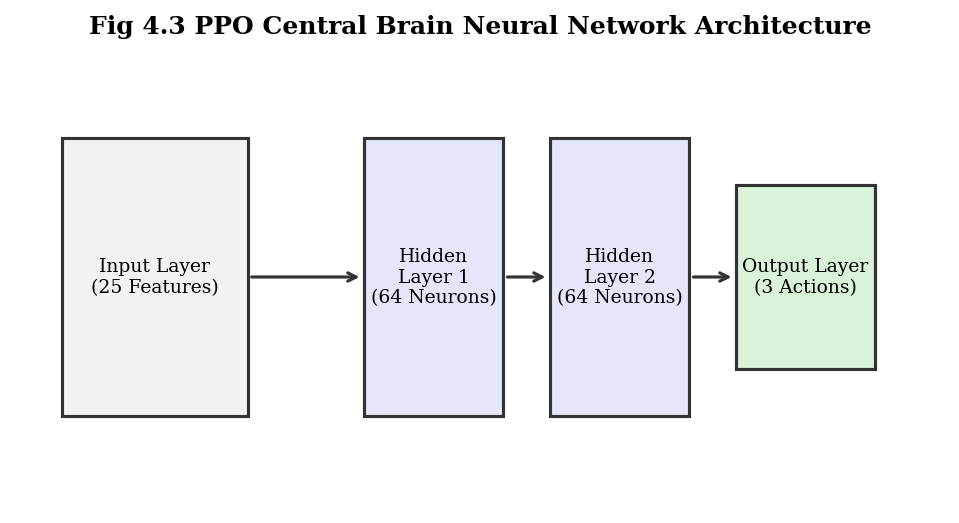
\includegraphics[width=0.85\textwidth]{images/fig4_3_ppo_architecture.png}
    \caption{PPO Central Brain Neural Network Architecture (MLP: 25 $\to$ 64 $\to$ 64 $\to$ 3)}
    \label{fig:ppo_arch}
\end{figure}

% ----------------------------------------------------------------
\subsection{Overfitting Mitigation: EvalCallback}

To prevent the trained model from overfitting to the specific conditions of the
training episodes and to ensure that the deployed model represents the peak of
generalization performance rather than just the final training checkpoint, an
\texttt{EvalCallback} is integrated into the training loop. Every 5,000 training
steps, the callback evaluates the current model on a held-out evaluation
environment for 5 full episodes and records the mean reward. If the mean reward
exceeds the previously recorded best, the current model is saved as
\texttt{best\_model.zip}. At the end of the 50,000-step training run, the
best-performing checkpoint is loaded and deployed into the benchmark simulation.

The entropy coefficient $ent\_coef = 0.01$ addresses underfitting on the other
end of the spectrum. Without exploration pressure, the PPO agent tends to converge
prematurely to a single routing strategy (typically Fuel-Priority) and stops
exploring RSL-Priority and Speed-Priority options. The entropy bonus maintains a
non-zero probability of selecting any action, preventing this collapse.

\begin{figure}[htbp]
    \centering
    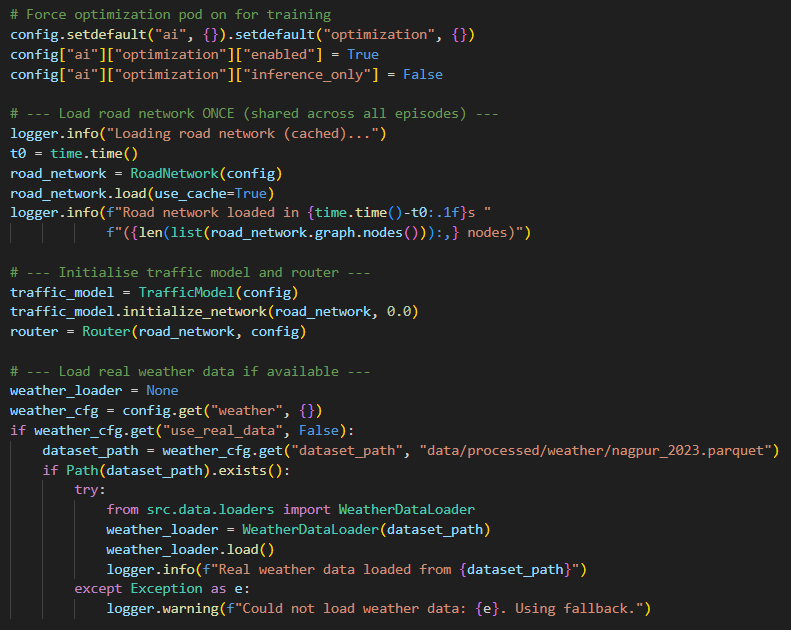
\includegraphics[width=0.95\textwidth, height=0.4\textheight, keepaspectratio]{images/screenshot_ppo_training_1.png}
    \vspace{0.2cm}
    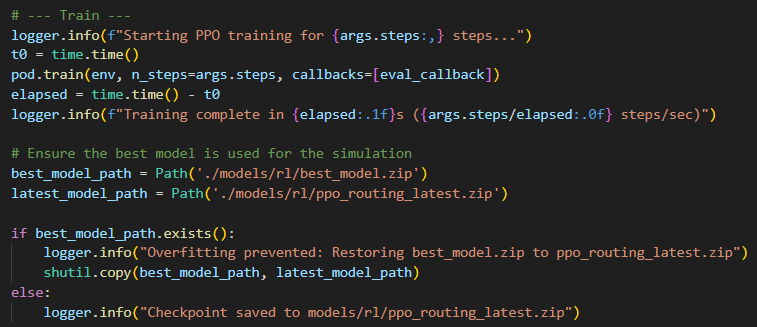
\includegraphics[width=0.95\textwidth, height=0.4\textheight, keepaspectratio]{images/screenshot_ppo_training_2.png}
    \caption{PPO Training Loop Implementation with EvalCallback for Overfitting Protection (Part 1 \& 2)}
    \label{fig:ppo_training_code}
\end{figure}

% ================================================================
\section{Anti-Thrashing GPS Lock}

% ----------------------------------------------------------------
\subsection{Discovery of the Route Thrashing Bug}

During initial integration testing, the combined system produced a delivery
service level of only 49.8\%, far below the 99.1\% achieved by the baseline
heuristic router. Analysis of the event logs revealed the cause: the Central PPO
Brain was broadcasting a strategy signal every 15 simulated minutes, and the truck
agent was interpreting each strategy signal as an instruction to recalculate its
entire route from scratch. Because the PPO agent was trained to broadcast the
Speed-Priority strategy frequently, trucks were continuously discarding their
current in-progress routes and spending the entire simulation recalculating paths
instead of driving them. The result was a fleet that was perpetually planning but
never delivering.

% ----------------------------------------------------------------
\subsection{The State Machine Fix}

The fix was implemented by adding a \texttt{\_last\_strategy\_action} state
variable to the truck agent. When a new strategy signal is received, the truck
compares it to the currently active strategy. If they match, the signal is ignored
and the truck continues on its current route. Only if the strategy has actually
changed does the truck trigger a route recalculation. This simple state machine
lock eliminated the thrashing behavior entirely.

Figure~\ref{fig:antithrash} illustrates the behavior before and after the fix.

\begin{figure}[h!]
    \centering
    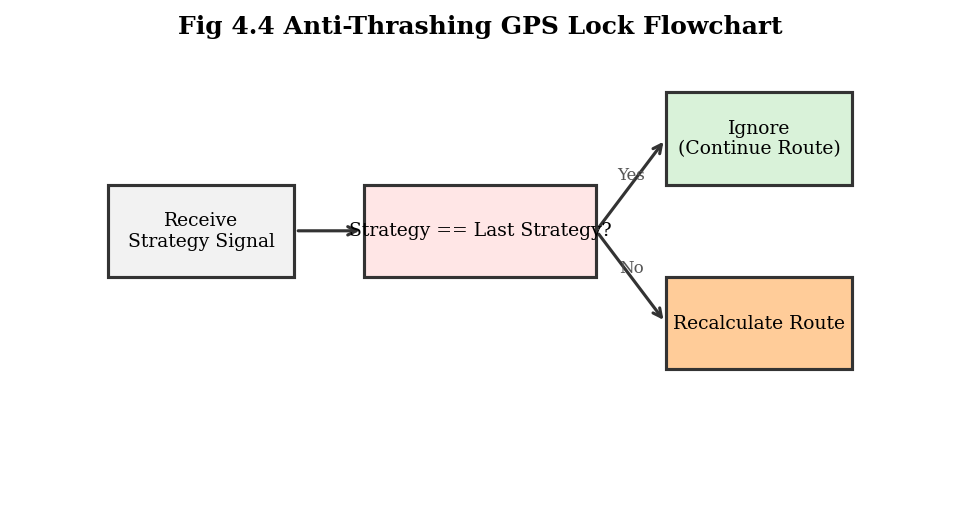
\includegraphics[width=0.95\textwidth]{images/fig4_4_antithrash.png}
    \caption{Anti-Thrashing GPS Lock: Behavior Before and After the Fix}
    \label{fig:antithrash}
\end{figure}

After applying the fix, the service level recovered to 99.9\%, confirming that the
underlying PPO policy was correct and that the thrashing bug had been the sole
cause of the performance collapse.

% ================================================================
\vspace{1cm}
\noindent \textbf{Chapter Summary:} This chapter described the implementation of
all five system components: the discrete-event simulation engine, the Nagpur city
graph, the three-tier AI architecture (Central PPO Brain, Edge Q-Agent, and ETA
Forecaster), the PPO training pipeline with EvalCallback, and the Anti-Thrashing
GPS Lock. Together, these components form a complete, production-quality AI-driven
supply chain optimization system. The next chapter presents the results of the
365-day benchmark that validates the system's performance.
